\section[Rastreabilidade de Requisitos]{Rastreabilidade de Requisitos}

Nessa seção estão descritas a rastreabilidade horizontal, vertical e a pré-rastreabilidade.


\subsection{Pré-Rastreabilidade}

Todos os requisitos identificados no projeto foram provenientes dos envolvidos.

% A rastreabilidade pode ser dividida em pré-rastreabilidade e pós-rastreabilidade. 
% A pré-rastreabilidade consiste no rastreamento de informações anteriores a especificação
% de requisitos. Como por exemplo, a fonte dos requisitos que podem ser: \textit{stakeholders},
% documentos e regras de negócio. Já a pós-rastreabilidade está relacionada com os requisitos depois 
% de serem especificados e está mais focada na solução. \cite{persson}
% 
% A rastreabilidade também pode ser horizontal ou vertical. A horizontal está relacionada com
% as informações de uma mesma fase do processo de desenvolvimento e a vertical
% com informações entre várias fases do processo. \cite{persson}
% 
% De acordo com \citeonline{paetsch}, a rastreabilidade auxilia na gerência de mudanças, 
% pois estabelece um relacionamento entre os requisitos, o projeto e a implementação do sistema. \citeonline{nuseibeh}
% afirmam que a rastreabilidade é o coração do gerenciamento de requisitos.
% 
% No SAFe os requisitos possuem quatro graus diferentes de abstração dos requisitos: tema de investimento, épicos, \textit{features} e histórias.
% A partir disso, a rastreabilidade definida para esse trabalho pode ser vista na Figura \ref{fig:rastreabilidade}.
% Será realizada uma rastreabilidade, através da ferramenta de gerenciamento de requisitos, vertical e horizontal. Assim acompanhando
% a origem das histórias, ou seja, de qual \textit{feature} e épico é derivada e também monitorar as dependências entre as histórias,\textit{features} e épicos.
% 
% Também será realizada a pré-rastreabilidade para identificar a fonte dos requisitos. A rastreabilidade definida será feita através da ferramenta de gerenciamento de requisitos.
% 
% \graphicspath{{figuras/}}
% 

\subsection{Rastreabilidade vertical}
A rastreabilidade dos requisitos entre o Tema de Investimento, Épicos e \textit{Features} pode ser vista na Figura \ref{fig:rastreabilidade}.
Já a matriz de rastreabilidade entre os épicos e \textit{features} pode ser vista na Figura \ref{fig:epft}. A rastreabilidade
entre as histórias e as \textit{features} podem ser vistas nas Figuras \ref{fig:ft01} e \ref{fig:ft04}. Todas as imagens foram geradas
na ferramenta TraceCloud. \footnotemark

\footnotetext{https://www.tracecloud.com/GloreeJava2/jsp/WebSite/TCHome.jsp}
\begin{figure}[!htb]
 \centering
 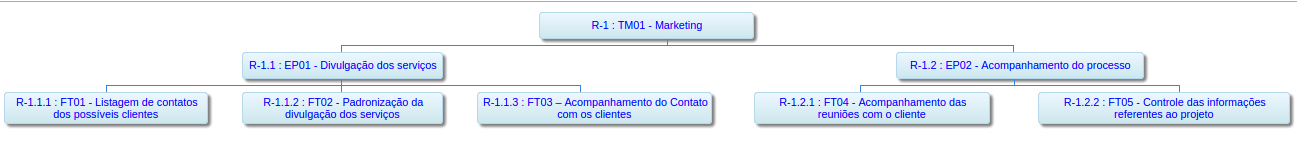
\includegraphics[scale= 0.5, angle=-90]{figuras/rastreabilidade_ferramenta.png}
 \caption{Rastreabilidade do Tema de investimento, épicos e \textit{features}}
 \label{fig:rastreabilidade}
\end{figure}

\begin{figure}[!htb]
 \centering
 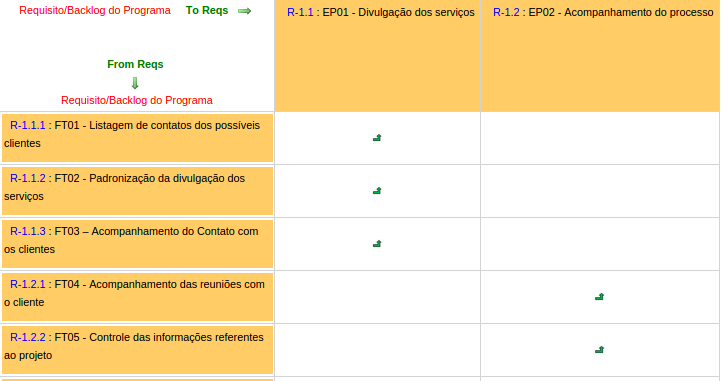
\includegraphics[scale= 0.5]{figuras/epft.png}
 \caption{Rastreabilidade dos épicos e \textit{features}}
 \label{fig:epft}
\end{figure}

\begin{figure}[!htb]
 \centering
 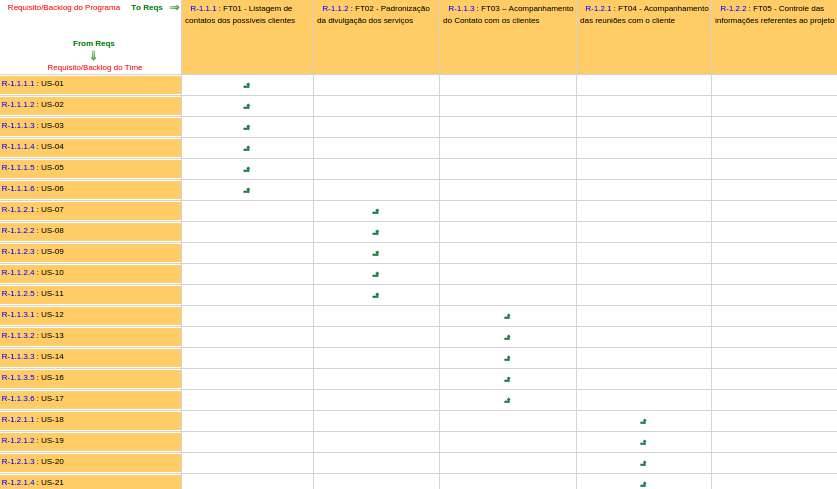
\includegraphics[scale= 0.5]{figuras/ft01e02.png}
 \caption{Rastreabilidade das histórias e \textit{features} 01, 02 e 03}
 \label{fig:ft01}
\end{figure}

\begin{figure}[!htb]
 \centering
 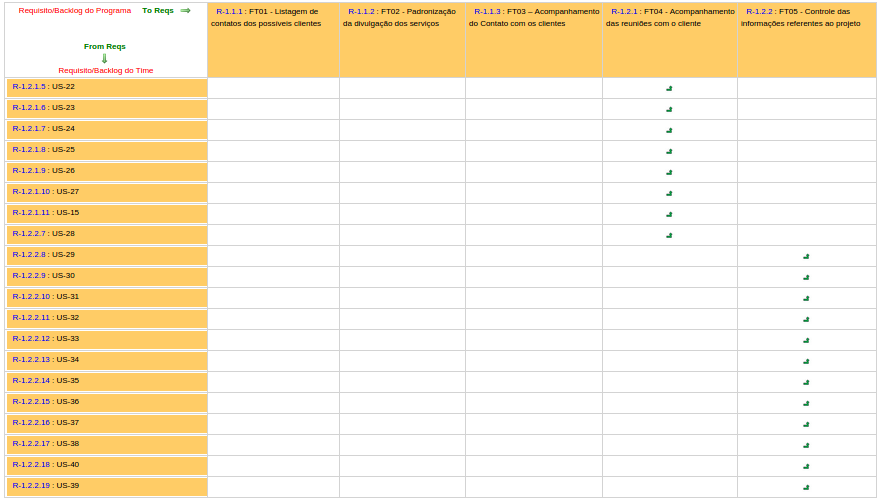
\includegraphics[scale= 0.5]{figuras/ft04e05.png}
 \caption{Rastreabilidade das histórias e \textit{features} 04 e 05}
 \label{fig:ft04}
\end{figure}
% \begin{figure}[!htb]
%  \centering
%  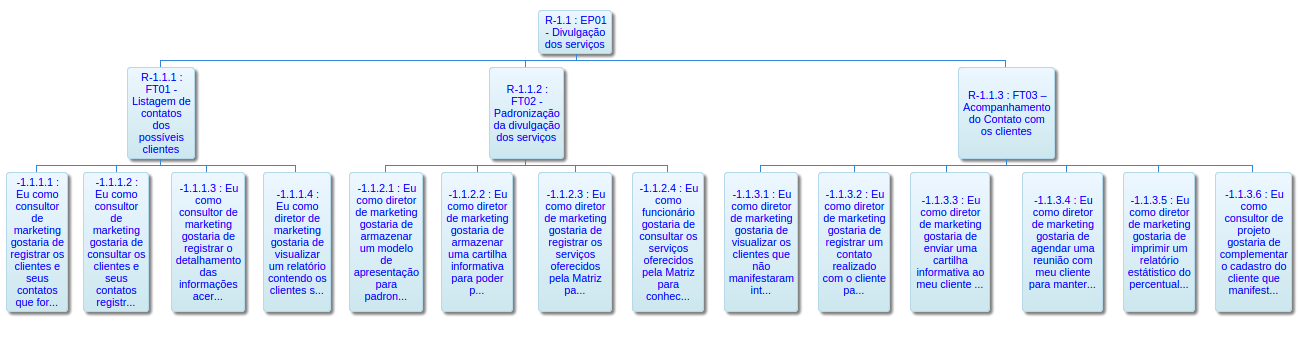
\includegraphics[scale= 0.5, angle=-90]{figuras/EP01.png}
%  \caption{Rastreabilidade do Épico 01, \textit{features} e histórias}
%  \label{rast2}
% \end{figure}
% 
% \begin{figure}[!htb]
%  \centering
%  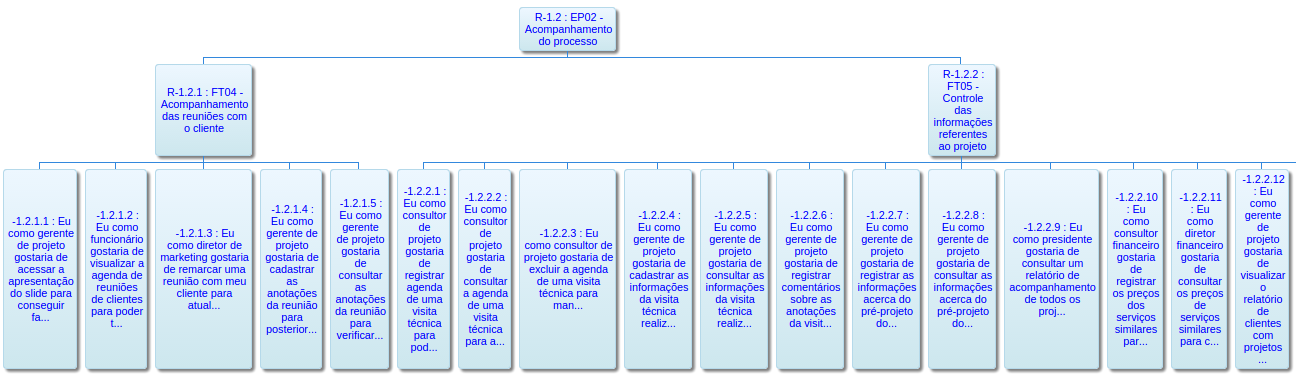
\includegraphics[scale= 0.5, angle=-90]{figuras/EP02.png}
%  \caption{Rastreabilidade do Épico 02, \textit{features} e histórias}
%  \label{rast3}
% \end{figure}

% \begin{figure}[!htb]
%  \centering
%  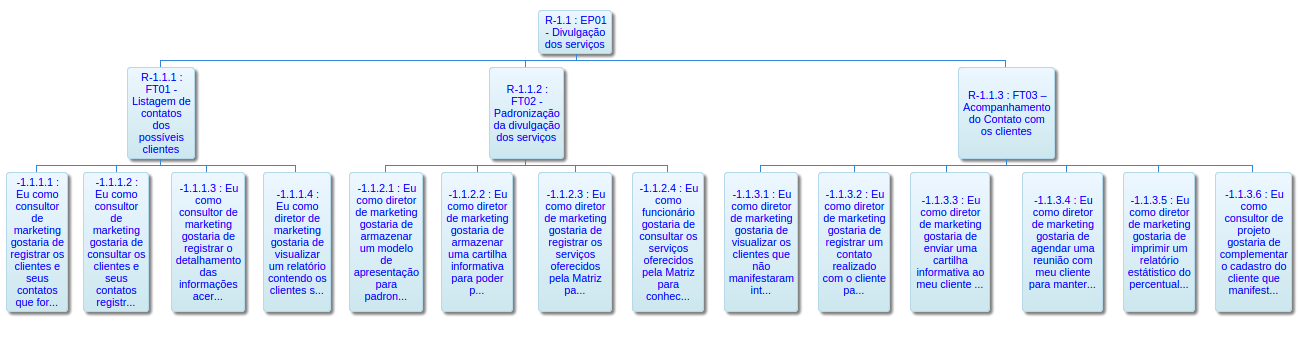
\includegraphics[scale= 0.5, angle=-90]{figuras/EP01.png}
%  \caption{Rastreabilidade do Épico 01, \textit{features} e histórias}
%  \label{rast2}
% \end{figure}
% 
% \begin{figure}[!htb]
%  \centering
%  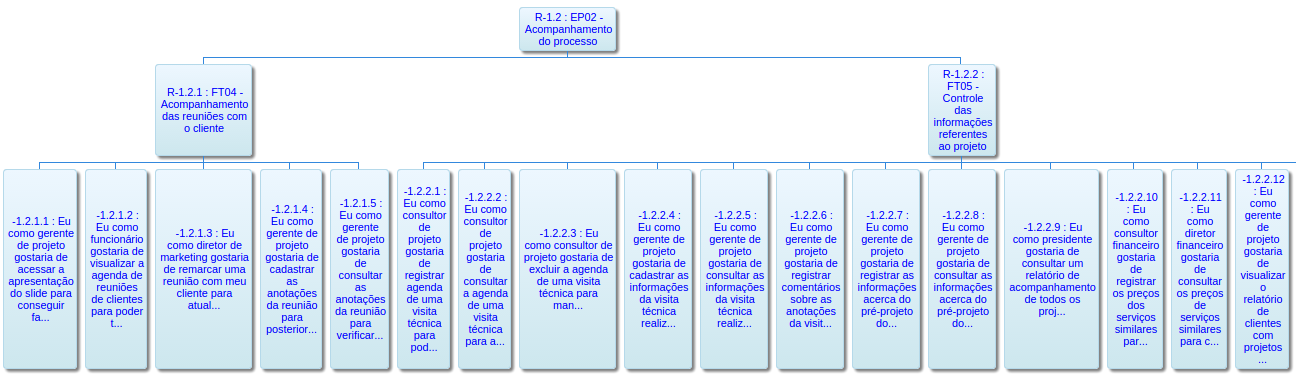
\includegraphics[scale= 0.5, angle=-90]{figuras/EP02.png}
%  \caption{Rastreabilidade do Épico 02, \textit{features} e histórias}
%  \label{rast3}
% \end{figure}

\subsection{Rastreabilidade horizontal}

Na tabela \ref{horizontal} podem-ser vistas as dependências entre as \textit{Features} e na tabela \ref{horizontal2} as dependências
entre as histórias

\begin{table*}[!h]
\centering
\label{horizontal}
\caption{Rastreabilidade horizontal dos requisitos - \textit{Features}}
\begin{tabular}{p{0.20\linewidth}p{0.20\linewidth}}
  \hline
  \textit{Feature}  & Dependência \\
  \hline
      FT03& FT01\\
      FT04& FT03 \\
      FT05& FT04 \\
  \hline
  \end{tabular}
\\
\label{horizontal2}
\caption{Rastreabilidade horizontal dos requisitos - Histórias}
\begin{tabular}{p{0.20\linewidth}p{0.20\linewidth}}
  \hline
  História  & Dependência \\
  \hline
      US-02 & US-01\\
      US-03 & US-01\\
      US-04 & US-02\\
      US-05 & US-02\\
      US-06 & US-02\\
      US-10 & US-09\\
      US-11 & US-09\\
      US-12 & US-13\\
      US-14 & US-08\\
      US-16 & US-13\\
      US-17 & US-13\\
      US-18 & US-07\\
      US-19 & US-15\\
      US-20 & US-15\\
      US-22 & US-21\\
      US-24 & US-23\\
      US-25 & US-23\\
      US-26 & US-23\\
      US-28 & US-27\\
      US-31 & US-30\\
      US-32 & US-30\\
      US-35 & US-34\\
      US-36 & US-34\\ 
   \hline
  \end{tabular}
\end{table*}



